% Options for packages loaded elsewhere
\PassOptionsToPackage{unicode}{hyperref}
\PassOptionsToPackage{hyphens}{url}
%
\documentclass[
  10pt,
]{article}
\usepackage{amsmath,amssymb}
\usepackage{lmodern}
\usepackage{iftex}
\ifPDFTeX
  \usepackage[T1]{fontenc}
  \usepackage[utf8]{inputenc}
  \usepackage{textcomp} % provide euro and other symbols
\else % if luatex or xetex
  \usepackage{unicode-math}
  \defaultfontfeatures{Scale=MatchLowercase}
  \defaultfontfeatures[\rmfamily]{Ligatures=TeX,Scale=1}
\fi
% Use upquote if available, for straight quotes in verbatim environments
\IfFileExists{upquote.sty}{\usepackage{upquote}}{}
\IfFileExists{microtype.sty}{% use microtype if available
  \usepackage[]{microtype}
  \UseMicrotypeSet[protrusion]{basicmath} % disable protrusion for tt fonts
}{}
\makeatletter
\@ifundefined{KOMAClassName}{% if non-KOMA class
  \IfFileExists{parskip.sty}{%
    \usepackage{parskip}
  }{% else
    \setlength{\parindent}{0pt}
    \setlength{\parskip}{6pt plus 2pt minus 1pt}}
}{% if KOMA class
  \KOMAoptions{parskip=half}}
\makeatother
\usepackage{xcolor}
\IfFileExists{xurl.sty}{\usepackage{xurl}}{} % add URL line breaks if available
\IfFileExists{bookmark.sty}{\usepackage{bookmark}}{\usepackage{hyperref}}
\hypersetup{
  hidelinks,
  pdfcreator={LaTeX via pandoc}}
\urlstyle{same} % disable monospaced font for URLs
\usepackage[margin=1in]{geometry}
\usepackage{color}
\usepackage{fancyvrb}
\newcommand{\VerbBar}{|}
\newcommand{\VERB}{\Verb[commandchars=\\\{\}]}
\DefineVerbatimEnvironment{Highlighting}{Verbatim}{commandchars=\\\{\}}
% Add ',fontsize=\small' for more characters per line
\usepackage{framed}
\definecolor{shadecolor}{RGB}{248,248,248}
\newenvironment{Shaded}{\begin{snugshade}}{\end{snugshade}}
\newcommand{\AlertTok}[1]{\textcolor[rgb]{0.94,0.16,0.16}{#1}}
\newcommand{\AnnotationTok}[1]{\textcolor[rgb]{0.56,0.35,0.01}{\textbf{\textit{#1}}}}
\newcommand{\AttributeTok}[1]{\textcolor[rgb]{0.77,0.63,0.00}{#1}}
\newcommand{\BaseNTok}[1]{\textcolor[rgb]{0.00,0.00,0.81}{#1}}
\newcommand{\BuiltInTok}[1]{#1}
\newcommand{\CharTok}[1]{\textcolor[rgb]{0.31,0.60,0.02}{#1}}
\newcommand{\CommentTok}[1]{\textcolor[rgb]{0.56,0.35,0.01}{\textit{#1}}}
\newcommand{\CommentVarTok}[1]{\textcolor[rgb]{0.56,0.35,0.01}{\textbf{\textit{#1}}}}
\newcommand{\ConstantTok}[1]{\textcolor[rgb]{0.00,0.00,0.00}{#1}}
\newcommand{\ControlFlowTok}[1]{\textcolor[rgb]{0.13,0.29,0.53}{\textbf{#1}}}
\newcommand{\DataTypeTok}[1]{\textcolor[rgb]{0.13,0.29,0.53}{#1}}
\newcommand{\DecValTok}[1]{\textcolor[rgb]{0.00,0.00,0.81}{#1}}
\newcommand{\DocumentationTok}[1]{\textcolor[rgb]{0.56,0.35,0.01}{\textbf{\textit{#1}}}}
\newcommand{\ErrorTok}[1]{\textcolor[rgb]{0.64,0.00,0.00}{\textbf{#1}}}
\newcommand{\ExtensionTok}[1]{#1}
\newcommand{\FloatTok}[1]{\textcolor[rgb]{0.00,0.00,0.81}{#1}}
\newcommand{\FunctionTok}[1]{\textcolor[rgb]{0.00,0.00,0.00}{#1}}
\newcommand{\ImportTok}[1]{#1}
\newcommand{\InformationTok}[1]{\textcolor[rgb]{0.56,0.35,0.01}{\textbf{\textit{#1}}}}
\newcommand{\KeywordTok}[1]{\textcolor[rgb]{0.13,0.29,0.53}{\textbf{#1}}}
\newcommand{\NormalTok}[1]{#1}
\newcommand{\OperatorTok}[1]{\textcolor[rgb]{0.81,0.36,0.00}{\textbf{#1}}}
\newcommand{\OtherTok}[1]{\textcolor[rgb]{0.56,0.35,0.01}{#1}}
\newcommand{\PreprocessorTok}[1]{\textcolor[rgb]{0.56,0.35,0.01}{\textit{#1}}}
\newcommand{\RegionMarkerTok}[1]{#1}
\newcommand{\SpecialCharTok}[1]{\textcolor[rgb]{0.00,0.00,0.00}{#1}}
\newcommand{\SpecialStringTok}[1]{\textcolor[rgb]{0.31,0.60,0.02}{#1}}
\newcommand{\StringTok}[1]{\textcolor[rgb]{0.31,0.60,0.02}{#1}}
\newcommand{\VariableTok}[1]{\textcolor[rgb]{0.00,0.00,0.00}{#1}}
\newcommand{\VerbatimStringTok}[1]{\textcolor[rgb]{0.31,0.60,0.02}{#1}}
\newcommand{\WarningTok}[1]{\textcolor[rgb]{0.56,0.35,0.01}{\textbf{\textit{#1}}}}
\usepackage{longtable,booktabs,array}
\usepackage{calc} % for calculating minipage widths
% Correct order of tables after \paragraph or \subparagraph
\usepackage{etoolbox}
\makeatletter
\patchcmd\longtable{\par}{\if@noskipsec\mbox{}\fi\par}{}{}
\makeatother
% Allow footnotes in longtable head/foot
\IfFileExists{footnotehyper.sty}{\usepackage{footnotehyper}}{\usepackage{footnote}}
\makesavenoteenv{longtable}
\usepackage{graphicx}
\makeatletter
\def\maxwidth{\ifdim\Gin@nat@width>\linewidth\linewidth\else\Gin@nat@width\fi}
\def\maxheight{\ifdim\Gin@nat@height>\textheight\textheight\else\Gin@nat@height\fi}
\makeatother
% Scale images if necessary, so that they will not overflow the page
% margins by default, and it is still possible to overwrite the defaults
% using explicit options in \includegraphics[width, height, ...]{}
\setkeys{Gin}{width=\maxwidth,height=\maxheight,keepaspectratio}
% Set default figure placement to htbp
\makeatletter
\def\fps@figure{htbp}
\makeatother
\setlength{\emergencystretch}{3em} % prevent overfull lines
\providecommand{\tightlist}{%
  \setlength{\itemsep}{0pt}\setlength{\parskip}{0pt}}
\setcounter{secnumdepth}{5}
\usepackage{amsthm}
\usepackage{amsmath}
\usepackage{amssymb}
\usepackage{verbatim}
\usepackage{hyperref}
\usepackage[T1]{fontenc}
\usepackage[utf8]{inputenc}
\hypersetup{colorlinks,allcolors=blue}
\usepackage{enumerate}
\usepackage{lastpage}
\usepackage[shortlabels]{enumitem}
\usepackage{fancyhdr}
\pagestyle{fancy}
\fancyhf{}
\fancyhead[R]{Ingunn Lilja Bergsdóttir}
\fancyhead[C]{Heimaverkefni 1}
\fancyhead[L]{Hagnýt Bayesísk tölfræði}
\fancyfoot[L]{Háskóli Íslands}
\fancyfoot[R]{\thepage}
\usepackage{float}
\usepackage{algorithm}
\usepackage{algorithmicx}
\usepackage{algpseudocode}
\usepackage{caption}
\usepackage[sectionbib]{chapterbib}
\usepackage{booktabs}
\usepackage{longtable}
\usepackage{array}
\usepackage{multirow}
\usepackage{wrapfig}
\usepackage{float}
\usepackage{colortbl}
\usepackage{pdflscape}
\usepackage{tabu}
\usepackage{threeparttable}
\usepackage{threeparttablex}
\usepackage[normalem]{ulem}
\usepackage{makecell}
\usepackage{xcolor}
\ifLuaTeX
  \usepackage{selnolig}  % disable illegal ligatures
\fi

\author{}
\date{\vspace{-2.5em}}

\begin{document}

\hypertarget{other-exercises-1}{%
\section*{Other exercises 1}\label{other-exercises-1}}
\addcontentsline{toc}{section}{Other exercises 1}

\hypertarget{b}{%
\subsection*{(b)}\label{b}}
\addcontentsline{toc}{subsection}{(b)}

\begin{Shaded}
\begin{Highlighting}[]
\NormalTok{theta }\OtherTok{\textless{}{-}} \FunctionTok{seq}\NormalTok{(}\DecValTok{0}\NormalTok{,}\DecValTok{1}\NormalTok{,}\FloatTok{0.1}\NormalTok{)}
\NormalTok{y }\OtherTok{\textless{}{-}} \DecValTok{57}
\NormalTok{n }\OtherTok{\textless{}{-}} \DecValTok{100}

\NormalTok{bin\_fall }\OtherTok{\textless{}{-}} \ControlFlowTok{function}\NormalTok{(theta) \{}
  \FunctionTok{choose}\NormalTok{(n,y)}\SpecialCharTok{*}\NormalTok{theta}\SpecialCharTok{\^{}}\NormalTok{y}\SpecialCharTok{*}\NormalTok{(}\DecValTok{1}\SpecialCharTok{{-}}\NormalTok{theta)}\SpecialCharTok{\^{}}\NormalTok{(n}\SpecialCharTok{{-}}\NormalTok{y)}
\NormalTok{\}}

\NormalTok{results }\OtherTok{\textless{}{-}} \FunctionTok{tibble}\NormalTok{(theta, }\AttributeTok{bin =} \FunctionTok{sapply}\NormalTok{(theta, bin\_fall))}

\NormalTok{results }\SpecialCharTok{\%\textgreater{}\%}
  \FunctionTok{ggplot}\NormalTok{(}\FunctionTok{aes}\NormalTok{(theta, bin)) }\SpecialCharTok{+} 
  \FunctionTok{geom\_point}\NormalTok{() }\SpecialCharTok{+}
  \FunctionTok{labs}\NormalTok{(}\AttributeTok{x=}\FunctionTok{TeX}\NormalTok{(}\StringTok{"$}\SpecialCharTok{\textbackslash{}\textbackslash{}}\StringTok{theta$"}\NormalTok{),}
       \AttributeTok{y =} \StringTok{"Point mass"}\NormalTok{,}
       \AttributeTok{title =} \FunctionTok{TeX}\NormalTok{(}\StringTok{"Point mass at each value of $}\SpecialCharTok{\textbackslash{}\textbackslash{}}\StringTok{theta$"}\NormalTok{)) }\SpecialCharTok{+}
  \FunctionTok{theme\_classic}\NormalTok{()}
\end{Highlighting}
\end{Shaded}

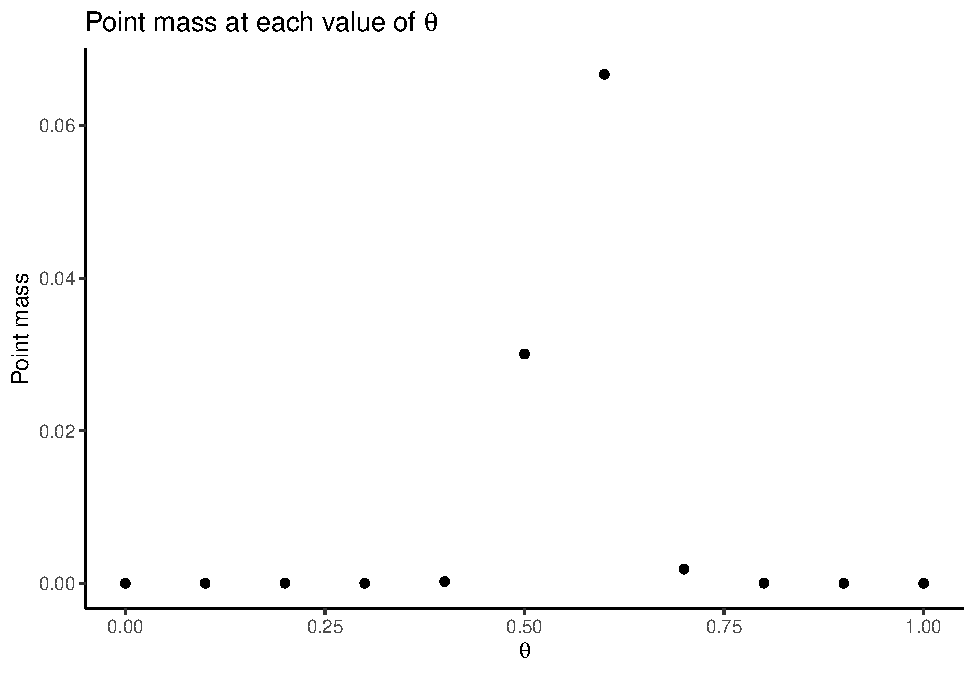
\includegraphics{Heimaverkefni-1_files/figure-latex/unnamed-chunk-1-1.pdf}

\hypertarget{c}{%
\subsection*{(c)}\label{c}}
\addcontentsline{toc}{subsection}{(c)}

Using Bayes rule we get that the posterior distribution for each theta is the point mass calculated in part \((b)\) divided by the sum of the beta values. This gives

\begin{Shaded}
\begin{Highlighting}[]
\CommentTok{\# sum up previous results}
\NormalTok{sum\_bin }\OtherTok{\textless{}{-}}\NormalTok{ results }\SpecialCharTok{\%\textgreater{}\%} 
  \FunctionTok{select}\NormalTok{(bin) }\SpecialCharTok{\%\textgreater{}\%} \FunctionTok{sum}\NormalTok{()}

\NormalTok{bin\_posterior }\OtherTok{\textless{}{-}} \ControlFlowTok{function}\NormalTok{(bin) \{bin}\SpecialCharTok{/}\NormalTok{sum\_bin\}}

\NormalTok{results\_posterior }\OtherTok{\textless{}{-}} \FunctionTok{tibble}\NormalTok{(theta, }\AttributeTok{bin\_post =} \FunctionTok{sapply}\NormalTok{(results}\SpecialCharTok{$}\NormalTok{bin, bin\_posterior))}

\NormalTok{results\_posterior }\SpecialCharTok{\%\textgreater{}\%}
  \FunctionTok{ggplot}\NormalTok{(}\FunctionTok{aes}\NormalTok{(theta, bin\_post)) }\SpecialCharTok{+}
  \FunctionTok{geom\_point}\NormalTok{() }\SpecialCharTok{+} 
  \FunctionTok{theme\_classic}\NormalTok{() }\SpecialCharTok{+}
  \FunctionTok{labs}\NormalTok{(}\AttributeTok{x=}\FunctionTok{TeX}\NormalTok{(}\StringTok{"$}\SpecialCharTok{\textbackslash{}\textbackslash{}}\StringTok{theta$"}\NormalTok{),}
       \AttributeTok{y =} \StringTok{"Point mass"}\NormalTok{,}
       \AttributeTok{title =} \FunctionTok{TeX}\NormalTok{(}\StringTok{"Posterior distribution"}\NormalTok{))}
\end{Highlighting}
\end{Shaded}

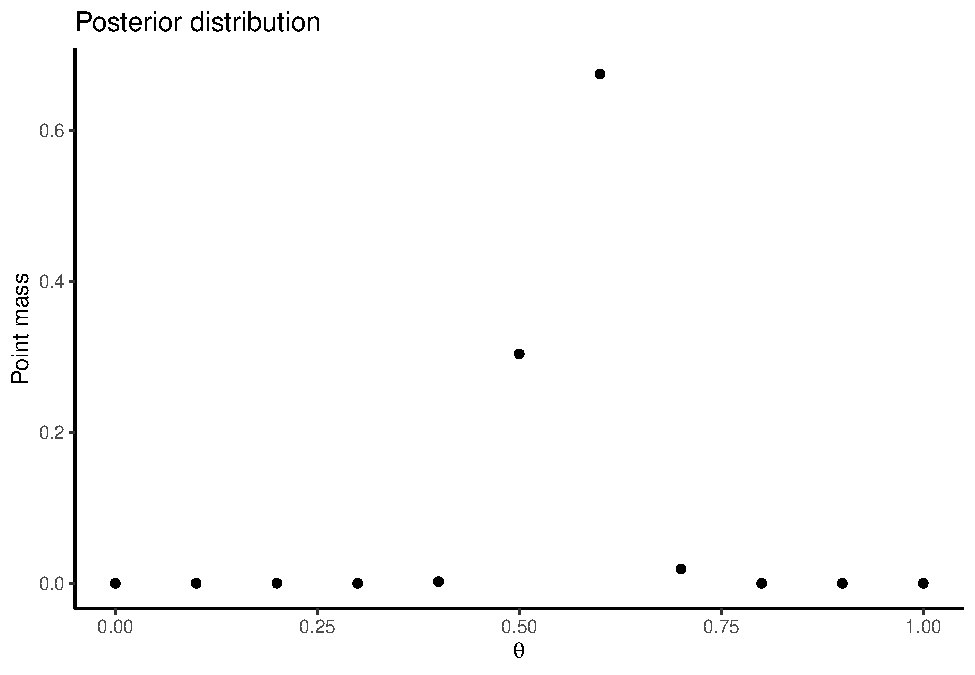
\includegraphics{Heimaverkefni-1_files/figure-latex/unnamed-chunk-2-1.pdf}

\hypertarget{d}{%
\subsection*{(d)}\label{d}}
\addcontentsline{toc}{subsection}{(d)}

Now suppose you allow \(\theta\) to be any value in the interval \([0,1]\). Using the uniform prior density for \(\theta\), so that \(p(\theta) = 1\), plot the posterior density of \(\theta\) as a function of \(\theta\). According to the posterior density, what is the probability of \(\theta > 0.5\)?

The uniform prior density is a special case of the beta distribution which is conjugate for the class of binomial sampling distributions
The uniform prior density can be set up as \(\theta^{1-1}(1-\theta)^{1-1}\) and we had the binomial likelihood \(\theta^y(1-\theta)^{n-y}\)
Bayes theorem then gives the parameters for the beta distribution \(\alpha = y+1\) and \(\beta = n-y+1\)

\begin{Shaded}
\begin{Highlighting}[]
\CommentTok{\# plot the beta distribution}
\NormalTok{theta }\OtherTok{\textless{}{-}} \FunctionTok{seq}\NormalTok{(}\DecValTok{0}\NormalTok{, }\DecValTok{1}\NormalTok{, }\FloatTok{0.0001}\NormalTok{)}

\FunctionTok{tibble}\NormalTok{(}\AttributeTok{x =}\NormalTok{ theta, }\AttributeTok{y =} \FunctionTok{dbeta}\NormalTok{(theta, }\AttributeTok{shape1 =} \DecValTok{57}\SpecialCharTok{+}\DecValTok{1}\NormalTok{, }\AttributeTok{shape2 =} \DecValTok{100{-}57}\SpecialCharTok{+}\DecValTok{1}\NormalTok{)) }\SpecialCharTok{\%\textgreater{}\%}
  \FunctionTok{ggplot}\NormalTok{(}\FunctionTok{aes}\NormalTok{(}\AttributeTok{x=}\NormalTok{x, }\AttributeTok{y =}\NormalTok{ y)) }\SpecialCharTok{+}
  \FunctionTok{geom\_line}\NormalTok{() }\SpecialCharTok{+}
  \FunctionTok{theme\_classic}\NormalTok{() }\SpecialCharTok{+} 
  \FunctionTok{labs}\NormalTok{(}\AttributeTok{x=}\FunctionTok{TeX}\NormalTok{(}\StringTok{"$}\SpecialCharTok{\textbackslash{}\textbackslash{}}\StringTok{theta$"}\NormalTok{),}
       \AttributeTok{y=}\FunctionTok{TeX}\NormalTok{(}\StringTok{"Posterior density of $}\SpecialCharTok{\textbackslash{}\textbackslash{}}\StringTok{theta$"}\NormalTok{),}
       \AttributeTok{title=}\FunctionTok{TeX}\NormalTok{(}\StringTok{"Posterior density for continuous $}\SpecialCharTok{\textbackslash{}\textbackslash{}}\StringTok{theta$"}\NormalTok{))}
\end{Highlighting}
\end{Shaded}

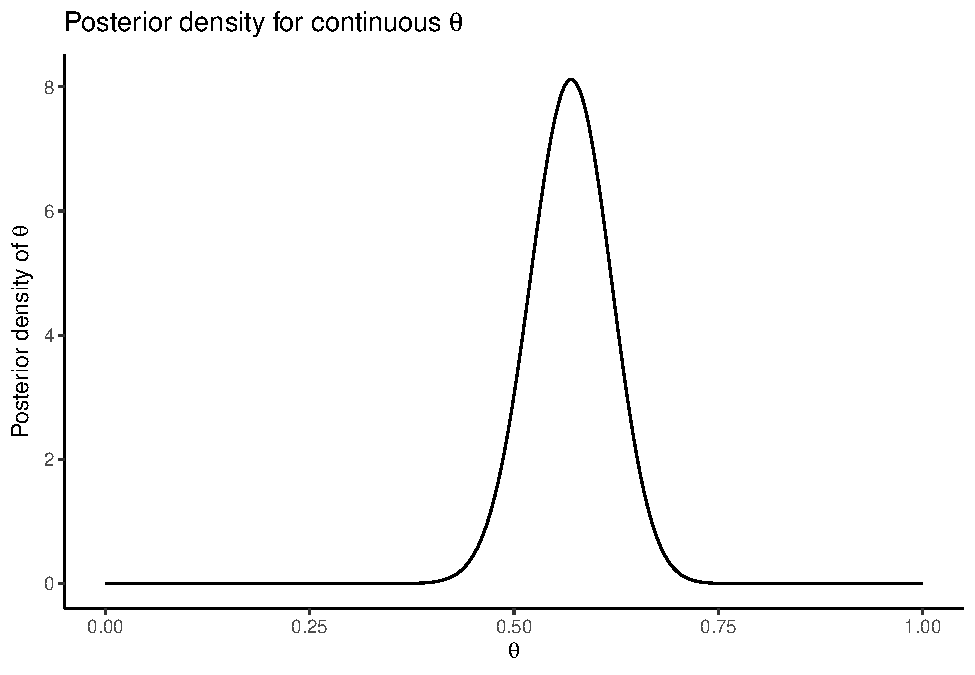
\includegraphics{Heimaverkefni-1_files/figure-latex/unnamed-chunk-3-1.pdf}

According to the posterior density what is the prob. of \(\theta > 0.5\) ?

\begin{Shaded}
\begin{Highlighting}[]
\DecValTok{1}\SpecialCharTok{{-}}\FunctionTok{pbeta}\NormalTok{(}\FloatTok{0.5}\NormalTok{, }\DecValTok{58}\NormalTok{, }\DecValTok{44}\NormalTok{)}
\end{Highlighting}
\end{Shaded}

\begin{verbatim}
## [1] 0.9183604
\end{verbatim}

\hypertarget{e}{%
\subsection*{(e)}\label{e}}
\addcontentsline{toc}{subsection}{(e)}

Why are the heights of posterior densities in (c) and (d) not the same?

The continuous \(\theta\) values reach 0.57, the maximum height, which the discrete \(\theta\) does not, therefore it goes higher.

\hypertarget{other-excercises-2}{%
\section*{Other excercises 2}\label{other-excercises-2}}
\addcontentsline{toc}{section}{Other excercises 2}

\hypertarget{random-numbers-probability-density-functions-pdf-and-cumulative-density-functionscdf}{%
\subsection*{Random numbers, probability density functions (pdf) and cumulative density functions(cdf)}\label{random-numbers-probability-density-functions-pdf-and-cumulative-density-functionscdf}}
\addcontentsline{toc}{subsection}{Random numbers, probability density functions (pdf) and cumulative density functions(cdf)}

The goal of this exercise is to generate random numbers, plot the histogram, the empirical pdf and cdf for these numbers, and see how they compare to the theoretical pdf and cdf. The goal is also to compare the sample mean and standard deviation to the theoretical mean and standard deviation.

\hypertarget{a}{%
\subsection*{(a)}\label{a}}
\addcontentsline{toc}{subsection}{(a)}

Generate \(B = 2000\) numbers from the gamma distribution with parameters \(\alpha = 3\) , \(\beta = 0.5\) (Matlab:gamrnd, R:rgamma). Compute the sample mean and the sample standard deviation and compare to the theoretical mean and standard deviation. (Matlab:mean,std, R:mean,sd).

\begin{Shaded}
\begin{Highlighting}[]
\FunctionTok{set.seed}\NormalTok{(}\DecValTok{2699}\NormalTok{)}

\NormalTok{n }\OtherTok{\textless{}{-}} \DecValTok{2000}
\NormalTok{alpha }\OtherTok{\textless{}{-}} \DecValTok{3}
\NormalTok{beta }\OtherTok{\textless{}{-}} \FloatTok{0.5}

\NormalTok{B }\OtherTok{\textless{}{-}} \FunctionTok{rgamma}\NormalTok{(}\DecValTok{2000}\NormalTok{, }\AttributeTok{shape =}\NormalTok{ alpha, }\AttributeTok{rate =} \FloatTok{0.5}\NormalTok{)}

\CommentTok{\# sample mean and sd}
\NormalTok{mean\_sample }\OtherTok{\textless{}{-}} \FunctionTok{mean}\NormalTok{(B)}
\NormalTok{sd\_sample }\OtherTok{\textless{}{-}} \FunctionTok{sd}\NormalTok{(B)}

\CommentTok{\# theoretical mean and sd}

\NormalTok{mean\_theo }\OtherTok{\textless{}{-}}\NormalTok{ alpha}\SpecialCharTok{/}\NormalTok{beta}
\NormalTok{sd\_theo }\OtherTok{\textless{}{-}} \FunctionTok{sqrt}\NormalTok{(alpha}\SpecialCharTok{/}\NormalTok{beta}\SpecialCharTok{\^{}}\DecValTok{2}\NormalTok{)}
\end{Highlighting}
\end{Shaded}

\begin{table}[!h]

\caption{\label{tab:unnamed-chunk-6} Comparison of means}
\centering
\begin{tabular}[t]{cc}
\toprule
\textbf{Sample mean} & \textbf{Theoretical mean}\\
\midrule
5.954974 & 6\\
\bottomrule
\end{tabular}
\end{table}

\begin{table}[!h]

\caption{\label{tab:unnamed-chunk-7} Comparison of standard deviations}
\centering
\begin{tabular}[t]{cc}
\toprule
\textbf{Sample sd} & \textbf{Theoretical sd}\\
\midrule
3.469081 & 3.464102\\
\bottomrule
\end{tabular}
\end{table}

\newpage

\hypertarget{b-1}{%
\subsection*{(b)}\label{b-1}}
\addcontentsline{toc}{subsection}{(b)}

Plot the theoretical density (pdf) of the gamma distribution (Matlab:gampdf, R:dgamma). Plotempirical density based on the data on the same graph. In Matlabksdensitycan be used. In R one can use densityplot(y) given that y are the data. Plot the histogram of the data on another graph (Matlab:hist, R:histogram).

\begin{Shaded}
\begin{Highlighting}[]
\FunctionTok{set.seed}\NormalTok{(}\DecValTok{2699}\NormalTok{)}

\CommentTok{\# theoretical density and empirical density}
\NormalTok{plot }\OtherTok{\textless{}{-}} \FunctionTok{tibble}\NormalTok{(}\AttributeTok{x =}\NormalTok{ B, }\AttributeTok{y =} \FunctionTok{dgamma}\NormalTok{(B,}\AttributeTok{shape =} \DecValTok{3}\NormalTok{, }\AttributeTok{rate =} \FloatTok{0.5}\NormalTok{))}

\NormalTok{plot }\SpecialCharTok{\%\textgreater{}\%}
  \FunctionTok{ggplot}\NormalTok{(}\FunctionTok{aes}\NormalTok{(}\AttributeTok{x=}\NormalTok{x, }\AttributeTok{y =}\NormalTok{ y)) }\SpecialCharTok{+}
  \FunctionTok{geom\_point}\NormalTok{(}\AttributeTok{size =} \FloatTok{0.1}\NormalTok{, }\AttributeTok{color =} \StringTok{"blue"}\NormalTok{) }\SpecialCharTok{+}
  \FunctionTok{theme\_classic}\NormalTok{() }\SpecialCharTok{+}
  \FunctionTok{labs}\NormalTok{(}\AttributeTok{x =} \StringTok{"rgamma \textasciitilde{} B"}\NormalTok{,}
       \AttributeTok{y =} \StringTok{"density"}\NormalTok{) }\SpecialCharTok{+}
  \FunctionTok{scale\_x\_continuous}\NormalTok{(}\AttributeTok{breaks =} \FunctionTok{seq}\NormalTok{(}\DecValTok{0}\NormalTok{, }\DecValTok{30}\NormalTok{, }\DecValTok{5}\NormalTok{)) }\OtherTok{{-}\textgreater{}}\NormalTok{ plot1}

\CommentTok{\# empirical density based on the data}
\FunctionTok{densityplot}\NormalTok{(B) }\OtherTok{{-}\textgreater{}}\NormalTok{ plot2}

\FunctionTok{plot\_grid}\NormalTok{(plot1, plot2)}
\end{Highlighting}
\end{Shaded}

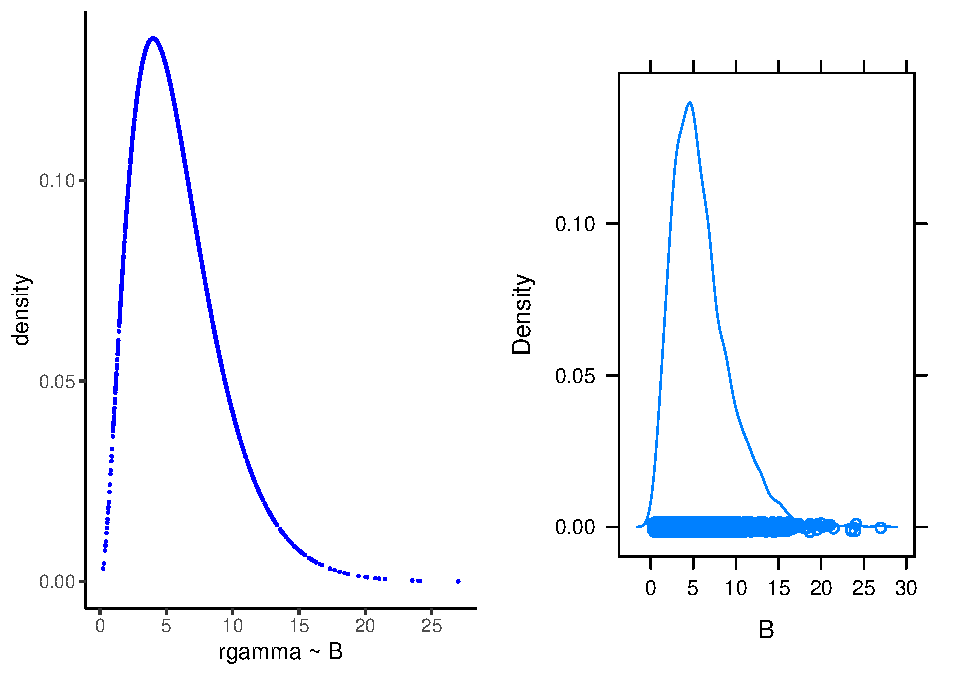
\includegraphics{Heimaverkefni-1_files/figure-latex/unnamed-chunk-8-1.pdf}
\newpage

\begin{Shaded}
\begin{Highlighting}[]
\CommentTok{\# Plot the histogram of the data on another graph}
\NormalTok{plot }\SpecialCharTok{\%\textgreater{}\%}
  \FunctionTok{ggplot}\NormalTok{(}\FunctionTok{aes}\NormalTok{(}\AttributeTok{x=}\NormalTok{x)) }\SpecialCharTok{+}
  \FunctionTok{geom\_histogram}\NormalTok{(}\AttributeTok{fill =} \StringTok{"blue"}\NormalTok{) }\SpecialCharTok{+}
  \FunctionTok{theme\_classic}\NormalTok{() }\SpecialCharTok{+}
  \FunctionTok{labs}\NormalTok{(}\AttributeTok{x =} \StringTok{"Gamma distributed data"}\NormalTok{,}
       \AttributeTok{y =} \StringTok{"count"}\NormalTok{) }\SpecialCharTok{+}
  \FunctionTok{scale\_x\_continuous}\NormalTok{(}\AttributeTok{breaks =} \FunctionTok{seq}\NormalTok{(}\DecValTok{0}\NormalTok{, }\DecValTok{30}\NormalTok{, }\DecValTok{5}\NormalTok{))}
\end{Highlighting}
\end{Shaded}

\begin{verbatim}
## `stat_bin()` using `bins = 30`. Pick better value with `binwidth`.
\end{verbatim}

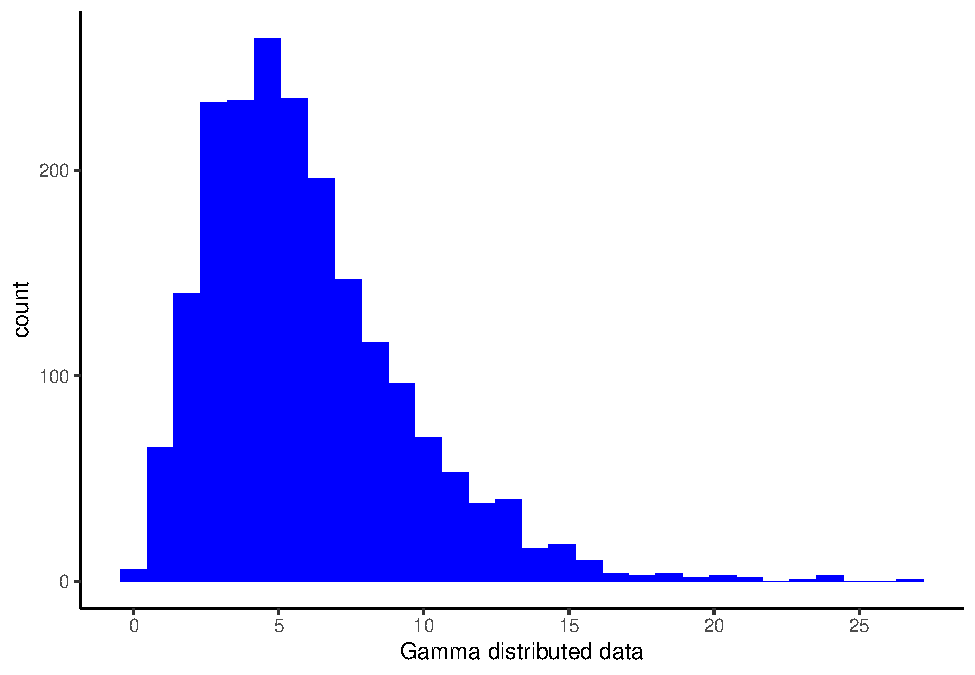
\includegraphics{Heimaverkefni-1_files/figure-latex/unnamed-chunk-9-1.pdf}

\hypertarget{c-1}{%
\subsection*{(c)}\label{c-1}}
\addcontentsline{toc}{subsection}{(c)}

Plot the theoretical cumulative density function (cdf) of the gamma distribution (Matlab:gamcdf, R:pgamma). Plot empirical cumulative density based on the data on the same graph.

\begin{Shaded}
\begin{Highlighting}[]
\FunctionTok{set.seed}\NormalTok{(}\DecValTok{2699}\NormalTok{)}

\CommentTok{\# heoretical cumulative density function (cdf) of the gamma distribution}
\NormalTok{plot }\OtherTok{\textless{}{-}} \FunctionTok{tibble}\NormalTok{(}\AttributeTok{x =}\NormalTok{ B,}
               \AttributeTok{y =} \FunctionTok{pgamma}\NormalTok{(B,}
                          \AttributeTok{shape =} \DecValTok{3}\NormalTok{,}
                          \AttributeTok{rate =} \FloatTok{0.5}\NormalTok{))}
\CommentTok{\# empirical density based on the data}
\NormalTok{n }\OtherTok{\textless{}{-}} \FunctionTok{length}\NormalTok{(B)}
\NormalTok{B\_sort }\OtherTok{\textless{}{-}} \FunctionTok{sort}\NormalTok{(B)}

\NormalTok{emp\_plot }\OtherTok{\textless{}{-}} \FunctionTok{tibble}\NormalTok{(}\AttributeTok{x=}\NormalTok{B\_sort,}
                   \AttributeTok{y=}\NormalTok{(}\DecValTok{1}\SpecialCharTok{:}\NormalTok{n)}\SpecialCharTok{/}\NormalTok{n)}

\NormalTok{plot }\SpecialCharTok{\%\textgreater{}\%}
  \FunctionTok{ggplot}\NormalTok{(}\FunctionTok{aes}\NormalTok{(}\AttributeTok{x=}\NormalTok{x, }\AttributeTok{y =}\NormalTok{ y)) }\SpecialCharTok{+}
  \FunctionTok{geom\_point}\NormalTok{(}\AttributeTok{size =} \FloatTok{0.1}\NormalTok{,}
             \AttributeTok{color =} \StringTok{"blue"}\NormalTok{) }\SpecialCharTok{+}
  \FunctionTok{theme\_classic}\NormalTok{() }\SpecialCharTok{+}
  \FunctionTok{labs}\NormalTok{(}\AttributeTok{x =} \StringTok{"rgamma \textasciitilde{} B"}\NormalTok{,}
       \AttributeTok{y =} \StringTok{"Density"}\NormalTok{) }\SpecialCharTok{+}
  \FunctionTok{scale\_x\_continuous}\NormalTok{(}\AttributeTok{breaks =} \FunctionTok{seq}\NormalTok{(}\DecValTok{0}\NormalTok{, }\DecValTok{30}\NormalTok{, }\DecValTok{5}\NormalTok{)) }\SpecialCharTok{+}
  \FunctionTok{geom\_point}\NormalTok{(}\AttributeTok{data =}\NormalTok{ emp\_plot,}
             \FunctionTok{aes}\NormalTok{(}\AttributeTok{x=}\NormalTok{x,}
                 \AttributeTok{y=}\NormalTok{y),}
             \AttributeTok{color =} \StringTok{"red"}\NormalTok{,}
             \AttributeTok{size =} \FloatTok{0.1}\NormalTok{) }\SpecialCharTok{+}
  \FunctionTok{annotate}\NormalTok{(}\AttributeTok{geom=}\StringTok{"text"}\NormalTok{, }\AttributeTok{x=}\FloatTok{2.5}\NormalTok{, }\AttributeTok{y=}\FloatTok{0.8}\NormalTok{, }\AttributeTok{label=}\StringTok{"empirical"}\NormalTok{, }\AttributeTok{color=}\StringTok{"red"}\NormalTok{) }\SpecialCharTok{+}
  \FunctionTok{annotate}\NormalTok{(}\AttributeTok{geom=}\StringTok{"text"}\NormalTok{, }\AttributeTok{x=}\FloatTok{2.5}\NormalTok{, }\AttributeTok{y=}\FloatTok{0.75}\NormalTok{, }\AttributeTok{label=}\StringTok{"pdf"}\NormalTok{, }\AttributeTok{color=}\StringTok{"blue"}\NormalTok{)}
\end{Highlighting}
\end{Shaded}

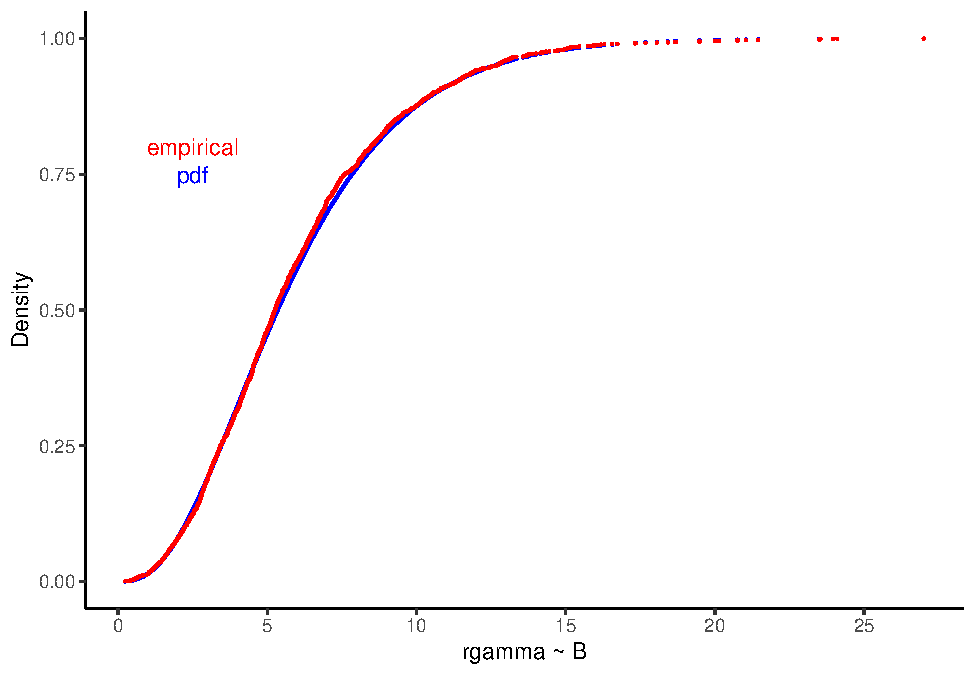
\includegraphics{Heimaverkefni-1_files/figure-latex/unnamed-chunk-10-1.pdf}

rgamma produces a well gamma distrubuted sample.

\end{document}
